\documentclass[conference]{IEEEtran}
\IEEEoverridecommandlockouts
% The preceding line is only needed to identify funding in the first footnote. If that is unneeded, please comment it out.
\usepackage{cite}
\usepackage{amsmath,amssymb,amsfonts}
\usepackage{algorithmic}
\usepackage{graphicx}
\usepackage{textcomp}
\usepackage{xcolor}
\usepackage{url}
\usepackage[colorlinks]{hyperref}
\usepackage{listings}
\usepackage{tikz}
\usepackage{tkz-euclide}
\usepackage{svg}

\usetikzlibrary{shapes,positioning}

\tikzset{ell/.style={circle,draw,minimum height=0.2cm,minimum width=0.2cm,inner sep=0.15cm}}


%New colors defined below
\definecolor{codegreen}{rgb}{0,0.6,0}
\definecolor{codegray}{rgb}{0.5,0.5,0.5}
\definecolor{codepurple}{rgb}{0.58,0,0.82}
\definecolor{backcolour}{rgb}{0.95,0.95,0.92}

%Code listing style named "mystyle"
\lstdefinestyle{mystyle}{
  backgroundcolor=\color{backcolour}, commentstyle=\color{codegreen},
  keywordstyle=\color{magenta},
  numberstyle=\tiny\color{codegray},
  stringstyle=\color{codepurple},
  basicstyle=\ttfamily\footnotesize,
  breakatwhitespace=false,         
  breaklines=true,                 
  captionpos=b,                    
  keepspaces=true,                 
  numbers=left,                    
  numbersep=5pt,                  
  showspaces=false,                
  showstringspaces=false,
  showtabs=false,                  
  tabsize=2
}

%"mystyle" code listing set
\lstset{style=mystyle}


\def\BibTeX{{\rm B\kern-.05em{\sc i\kern-.025em b}\kern-.08em
    T\kern-.1667em\lower.7ex\hbox{E}\kern-.125emX}}
\begin{document}

\title{Branch Prediction Models Exploration\\
\thanks{}
}
\author{\IEEEauthorblockN{Daniela Trevina}
\IEEEauthorblockA{\textit{Department of EECS} \\
\textit{Texas A\&M University-Kingsville}\\
Kingsville, USA \\
daniela.trevino@students.tamuk.edu}
\and
\IEEEauthorblockN{Daniela Lopez}
\IEEEauthorblockA{\textit{Department of EECS} \\
\textit{Texas A\&M University-Kingsville}\\
Kingsville, USA \\
daniela.lopez@students.tamuk.edu}
\and
\IEEEauthorblockN{Mengxiang Jiang}
\IEEEauthorblockA{\textit{Department of EECS} \\
\textit{Texas A\&M University-Kingsville}\\
Kingsville, USA \\
mengxiang.jiang@students.tamuk.edu}
\and
\IEEEauthorblockN{Samah Allahyani}
\IEEEauthorblockA{\textit{Department of EECS} \\
\textit{Texas A\&M University-Kingsville}\\
Kingsville, USA \\
samah.allahyani@students.tamuk.edu}
\and
\IEEEauthorblockN{Ugochukwu Onyeakazi}
\IEEEauthorblockA{\textit{Department of EECS} \\
\textit{Texas A\&M University-Kingsville}\\
Kingsville, USA \\
ugochukwu.onyeakazi@students.tamuk.edu}
}

\maketitle

\begin{abstract}
\end{abstract}

\section{Introduction}
Branch prediction is a crucial component in modern computer architecture to improve performance and energy efficiency. When executing a program, the processor encounters branches in the control flow, where it must decide which path to take based on a conditional statement. Incorrect branch predictions result in wasted computation cycles and negatively impact the overall performance of the system. To mitigate this issue, branch predictors are employed to predict the outcome of the conditional statements, and enable the processor to pre-fetch instructions from the predicted path, reducing the overhead of branching.

Over the years, a variety of branch prediction models have been developed to improve the accuracy of predictions. These models range from static branch predictors that use heuristics to predict the outcome of branches, to more sophisticated dynamic branch predictors (all models tested in this paper are dynamic) that rely on past history to make predictions. Furthermore, the emergence of  machine learning and artificial intelligence has led to the development of more advanced branch prediction techniques.

The aim of this paper is to explore the various branch prediction models and compare their performances. We will examine the underlying principles of each model, the algorithms used to make predictions and their implementations in a simulated processor. We will also discuss the challenges associated with branch prediction, such as the trade-off between prediction accuracy and hardware complexity.

\section{Models}
In this section, we will cover the various branch predictor models used in the simulation.

\subsection{Bimodal Predictor} \label{ssec::bimodal}
This model stores two bits in the branch target buffer (BTB) indicating whether this particular branch was taken or not taken the last two time. The bimodal branch predictor's accuracy will increase exponentially if the branch history size is increased. Most of the predictor's branches are taken or not taken and are not random. The main goal of this model is to distribute the branch behavior and predict which are the taken branches. The bimodal branch has a default size of a 2-bit counter which is organized in the low-order address-bit program counter section. When the branch is categorized as taken, the counter is increased. When the branch is categorized as not taken, then the counter is decreased. The counter value is limited and must be within the range of zero to three. This allows the branch predictor model to be categorized as taken or not taken using repeated values.


\subsection{Perceptron Predictor} \label{ssec:perceptron}
This model is a single-layer version of an artificial neural network that can identify and classify patterns, first applied to branch prediction by Jimenez and Lin\cite{jimenez2001dynamic}. In the model shown in Fig. \ref{fig:perceptron} are the input vector ($x$), the weight vector ($w$), and the output ($y$).
\begin{figure}
    \centering
    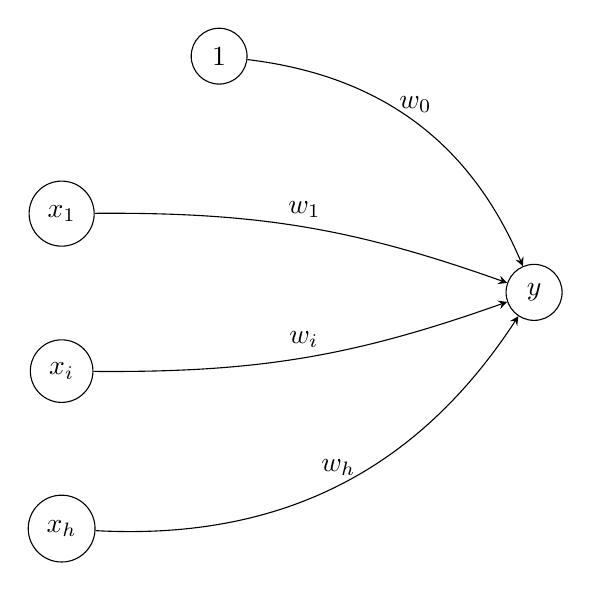
\begin{tikzpicture}[>=stealth]
		\node[ell] (x0) at (2,6) {$1$};
        \node[ell] (x1) at (0,4) {$x_1$};
        \node[ell] (xi) at (0,2) {$x_i$};
        \node[ell] (xh) at (0,0) {$x_h$};
        \node[ell] (y) at (6,3) {$y$};

        \draw [->] (x0) to [bend left]node[above]{$w_0$} (y);
		\draw [->] (x1) to [bend left=10]node[above]{$w_1$} (y);
		\draw [->] (xi) to [bend right=10]node[above]{$w_i$} (y);
		\draw [->] (xh) to [bend right]node[above]{$w_h$} (y);
    \end{tikzpicture}
    \caption{Perceptron Predictor}
	\label{fig:perceptron}
\end{figure}
The inputs correspond to values taken from the global history register, with the exception of $x_0$, the bias, always set to $1$. The output's sign determines the prediction. If the sign is negative, the branch is not taken, otherwise it is taken. Equation \eqref{eqn:1} shows the calculation of the output:
\begin{equation}
    y = w_o + \sum_{i=1}^{h}{x_iw_i}
    \label{eqn:1}
\end{equation}
\pagebreak
The weights of the perceptron are trained using the algorithm below:
\begin{lstlisting}
if sgn(y) != t or abs(y) <= theta  then
    for i := 0 to n do
        w[i] := w[i] + t*x[i]
    end
end
\end{lstlisting}
$t$ is 1 if the branch is actually taken or -1 if not. $\theta$ is the threshold to determine when training should stop. $w_i$ is incremented if $t$ and $x_i$ agree, and decremented if they disagree.

\subsection{Hashed Perceptron Predictor} \label{ssec::hp}
This predictor is based off of the perceptron branch predictor from the previous section(\ref{ssec:pp}) but with a few important changes. The first change is instead of a single table for the weights, multiple independently indexed tables of perceptron weights are used, introduced by Jimenez \cite{jimenez2003}.  The second is using the hash of the branch history rather than just the branch history for indexing in order to reduce the number of independent tables, contemporaneously by Seznec \cite{seznec2004}, Tarjan and Skadron\cite{skadron2004}, and Loh and Jimenez\cite{loh2005reducing}.  The third is instead of using a fixed history length, exponentially increasing history lengths are used for indexing, by Seznec\cite{seznec2004gehl}\cite{seznec2005analysis}. This idea is actually one of the key parts of the TAGE predictor described later. The last is dynamically adjust the $\theta$ value for the training, also by Seznec\cite{seznec2004gehl}\cite{seznec2005analysis}.


\bibliographystyle{plain}
\bibliography{project}

\vspace{12pt}

\end{document}
